\documentclass[10pt, uplatex, dvipdfmx]{jsarticle}
\usepackage{../mypackage}

\graphicspath{{../pictures}}

\setcounter{section}{4}

\begin{document}

\section{平面図形の面積と曲線の長さ}\label{sec:area}


\subsection{平面図形の面積と積分}

\begin{theorem}\label{thm:area}
  $f,g$ を有界閉区間 $[a,b]$ 上の連続関数とし,$[a,b]$ で $f(x) \geqq
  g(x)$ とする.図\ref{fig:area}のように曲
  線 $y=f(x)$ と$y=g(x)$ と $x$ 軸に垂直な $2$ 直線 $x=a, \, x=b$ で囲
  まれる有界閉領域
  \[
    D=\Set{(x,y) | a \leqq x \leqq b, \, g(x) \leqq y \leqq f(x)}
  \]
  の面積は以下の積分値に等しい.
  \[
    \int_{a}^{b} \left( f(x) - g(x) \right) dx
  \]
  \begin{figure}[h]
    \centering
    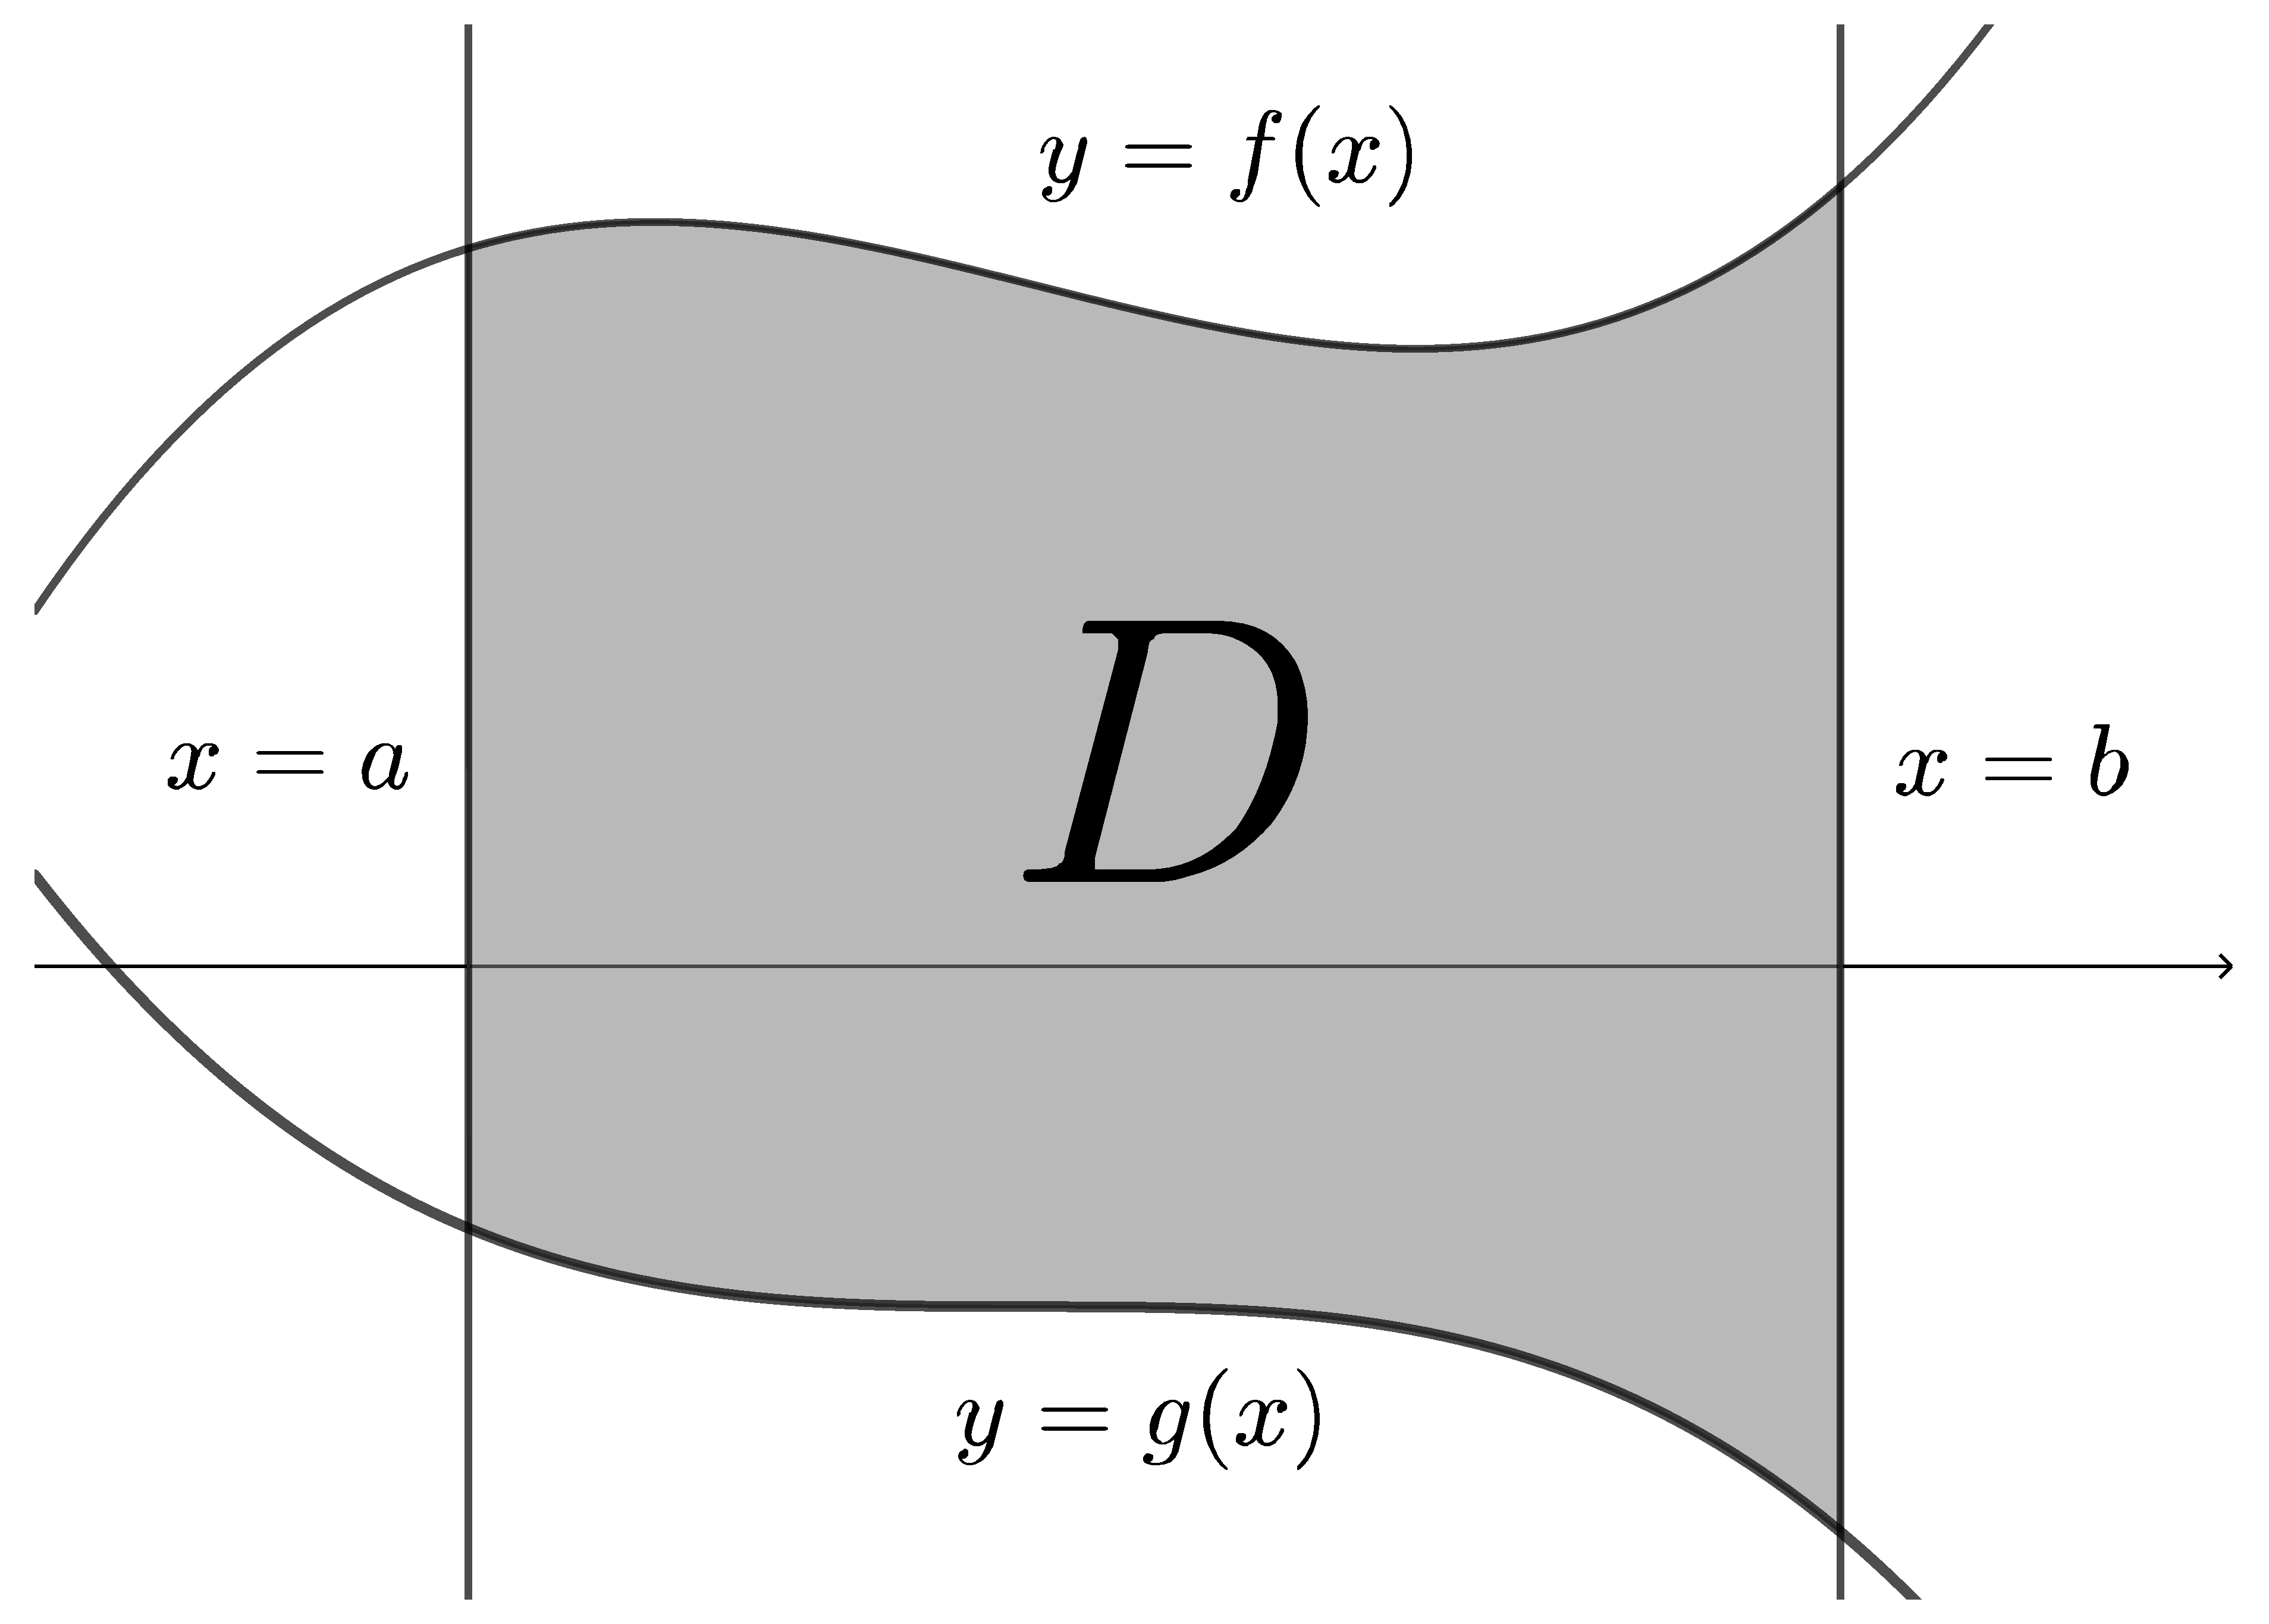
\includegraphics[width=7cm]{05/area.pdf}
    \caption{曲線 $y=f(x)$ と $y=g(x)$ と直線 $x=a$ と $x=b$ で囲まれる有界閉領域 $D$}
    \label{fig:area}
  \end{figure}
\end{theorem}


\begin{example}
  半径 $R>0$ の円の面積 $S(R)$ は図\ref{fig:circle}のように以下の積分で求められる.
  \[
    S(R) =\int_{-R}^{R} \left( \sqrt{R^2-x^2} - \left(-\sqrt{R^2-x^2}\right) \right) dx = \pi R^2
  \]
  \begin{figure}[h]
    \centering
    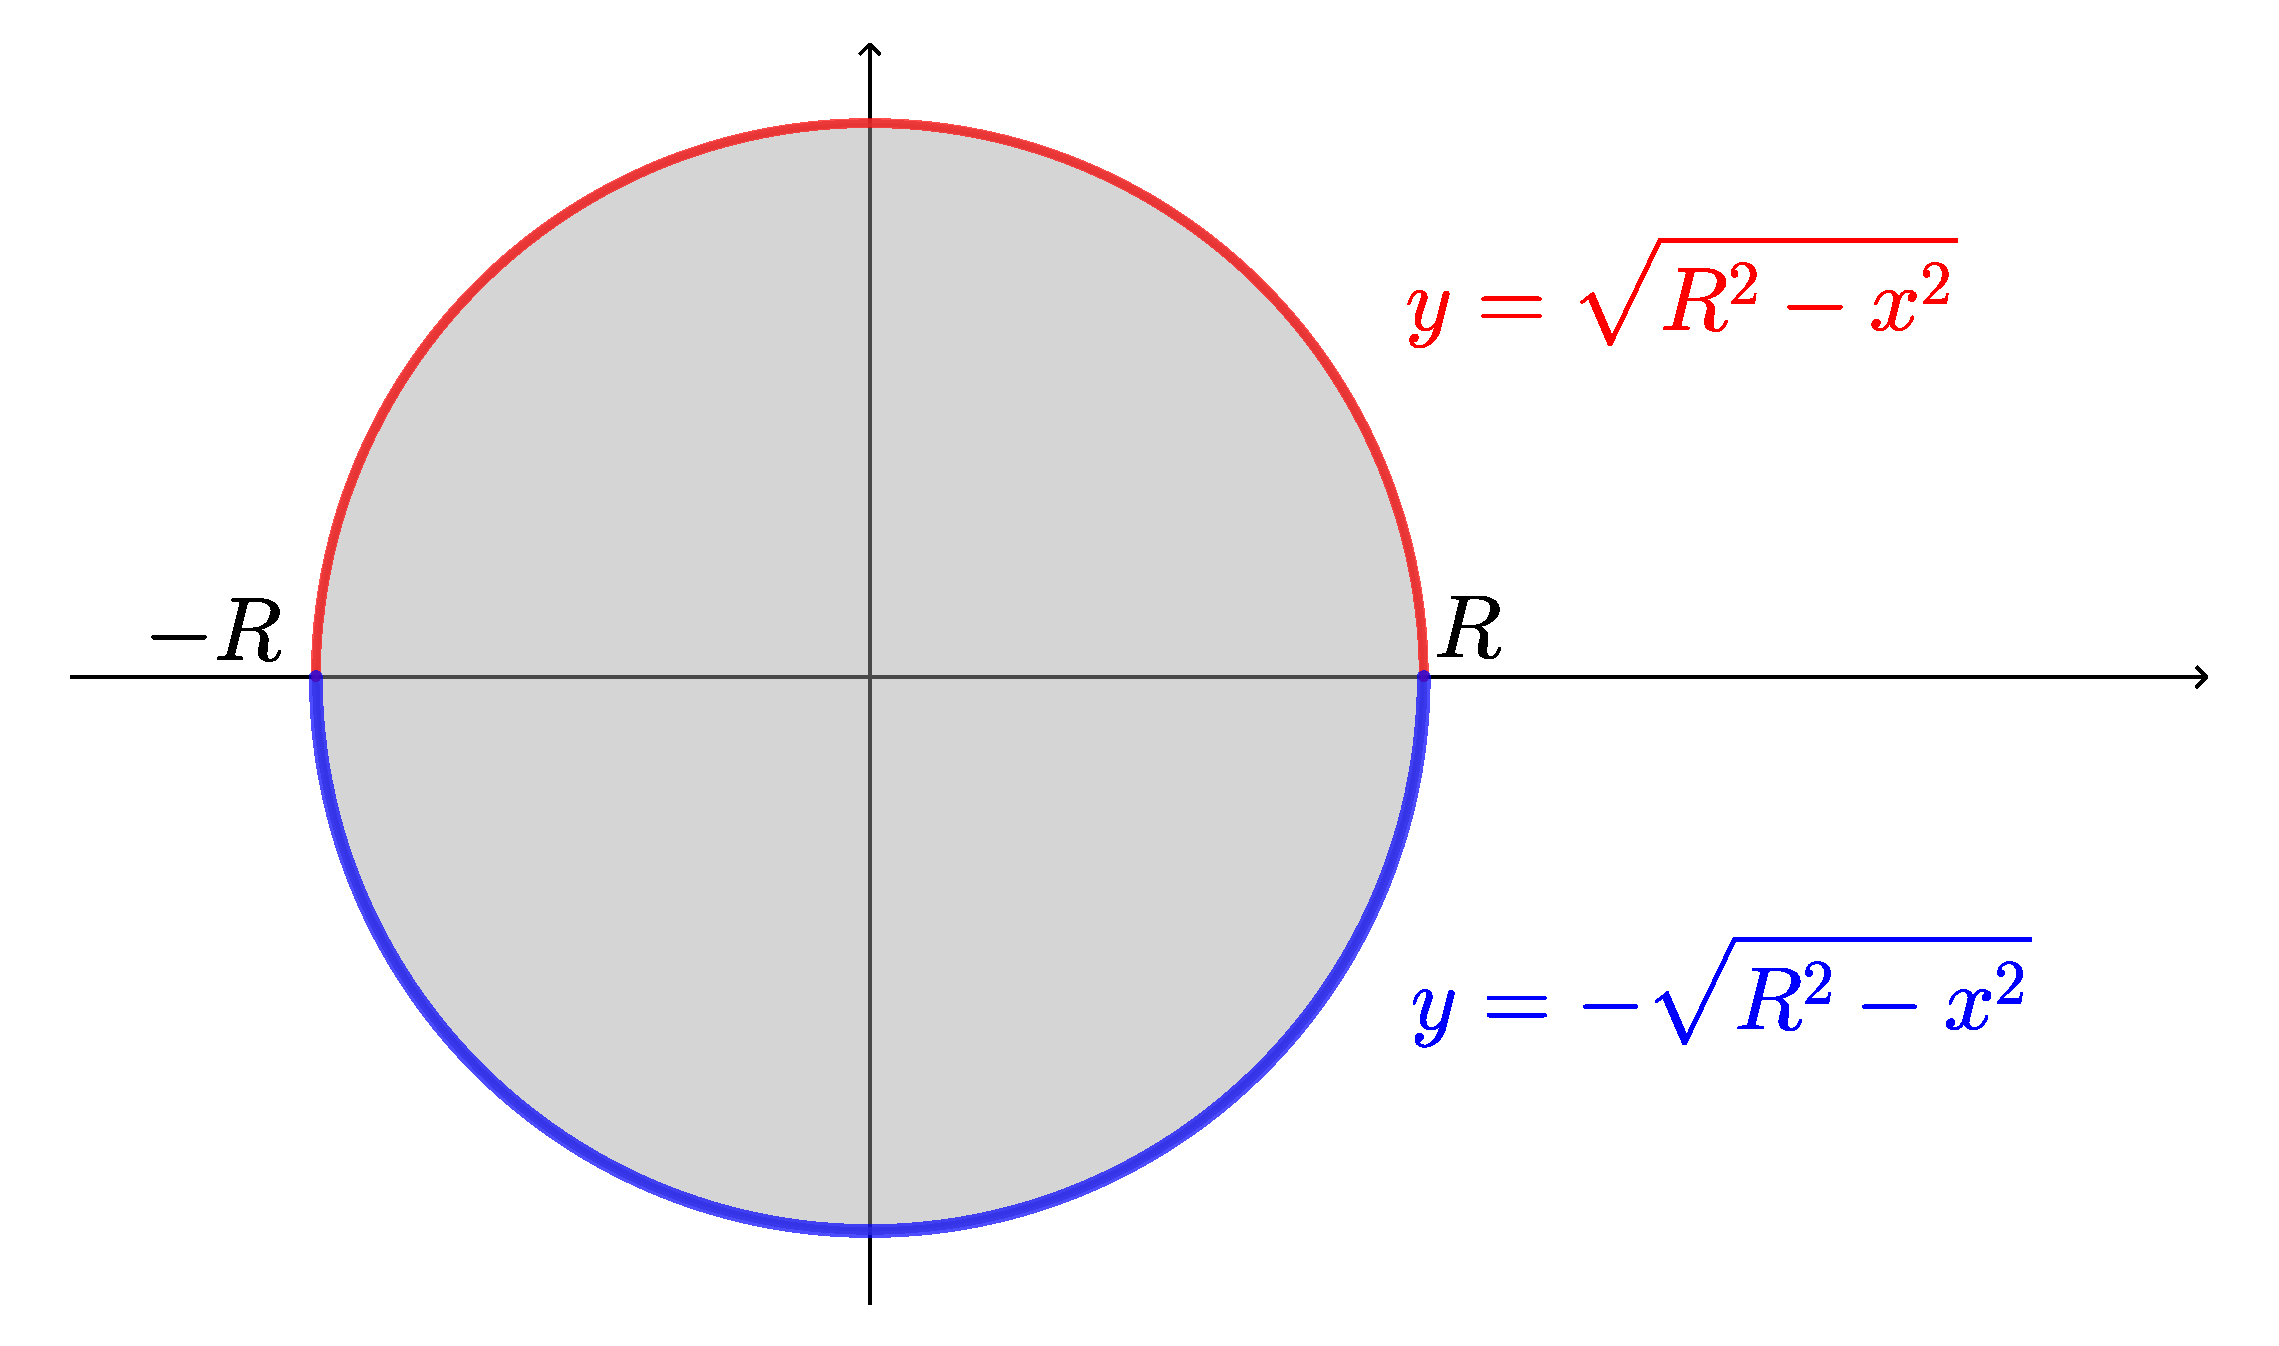
\includegraphics[width=8cm]{05/circle.pdf}
    \caption{曲線 $y=\pm \sqrt{R^2-x^2}$ と直
      線 $x= \pm R$ で囲まれる有界閉領域}
    \label{fig:circle}
  \end{figure}
\end{example}



\subsection{平面曲線の長さと積分}

積分を用いて曲線の長さを計算する.その前に「曲線の長さ」とは何かを定義
する.

$\varphi(t), \psi(t)$ を有界閉区間 $[a,b]$ 上定義された $C^1$ 級関数と
する.変数 $t$ が $a$ から $b$ まで動くとき,平面上の点
$\left( \varphi(t), \psi(t)\right)$ はなめらかな平面曲線 $C$ を描く.こ
れを
\[
  x=\varphi(t), \quad y=\psi(t), \quad a \leqq t \leqq b
\]
と書き,曲線 $C$
の\textbf{媒介変数表示}という.$\left( \varphi(a), \psi(a)\right), \,
\left(\varphi(b), \psi(b)\right)$ は $C$ の端点である.

曲線 $C$ を折れ線で近似する.閉区間 $[a,b]$ の分割
\[
  \Delta : a =t_0 < t_1 < t_2 < t_3< \cdots < t_{n-1} < t_n = b
\]
をとる.これにより曲線 $C$ 上に $n+1$ 個の点
$P_i\left( \varphi(t_i), \psi(t_i)\right) (i=0,1,\ldots, n)$ がとれる.
点 $P_0$ から $P_n$ までを順に結んで図\ref{fig:curve}のように曲線 $C$
を近似する折れ線ができる.
\begin{figure}[h]
  \centering
  \includegraphics[height=8cm]{05/curve.pdf}
  \caption{曲線 $C : x=\varphi(t), y=\psi(t)$ を近似する折れ線}
  \label{fig:curve}
\end{figure}

ここで
\[
\Delta x_i=\varphi(t_i)-\varphi(t_{i-1}), \quad \Delta y_i =\psi(t_i) - \psi(t_{i-1}), \quad
\Delta t_i = t_{i}-t_{i-1}
\]
とすれば,各線分 $P_{i-1}P_i$ の長さは三平方の定理から $\sqrt{{\Delta x_i}^2 + {\Delta
    y_i}^2}$ なので,$C$ を近似する折れ線の長さ $l_{\Delta}$ は次のように書ける.
\[
  l_{\Delta} = \sum_{i=1}^{n}\sqrt{{\Delta x_i}^2 + {\Delta y_i}^2} 
\]
そこで,$|\Delta| \to 0$ のときの $l_{\Delta}$ の極限値を曲線 $C$ の長
さと定義する.

次に,曲線 $C$ の長さ $\ds \lim_{|\Delta| \to 0} l_{\Delta}$ を積分を用
いて表す.まず,$l_{\Delta}$ は
\[
  \sqrt{{\Delta x_i}^2 + {\Delta y_i}^2} 
  =\sqrt{ \left(\frac{\Delta x_i}{\Delta
        t_i}\right)^2 + \left( \frac{\Delta y_i}{\Delta t_i}\right)^2
  }\ \Delta t_i
\]
と書ける.ここで,$\varphi, \psi$ は $C^1$ 級なので平均値の定理から
各 $i=1,2,\ldots, n$ に対して
\begin{align*}
  \frac{\Delta x_i}{\Delta t_i} = \frac{\varphi(t_i) - \varphi(t_{i-1})}{t_{i}-t_{i-1}} = \varphi'(c_i), \quad
  \frac{\Delta y_i}{\Delta t_i} = \frac{\psi(t_i) - \psi(t_{i-1})}{t_{i}-t_{i-1}} = \psi'(d_i)
\end{align*}
を満たす $c_i, d_i \in [t_{i-1}, t_{i}]$ が存在する.ここ
で,$\psi$ は $C^1$ 級と仮定したから $\psi'$ は連続である.よっ
て,$|\Delta| \to 0$のとき $d_i \to c_i$ なので $\psi'(d_i) \to
\psi'(c_i)$ である.従って,
\begin{align*}
  \lim_{|\Delta| \to 0} l_{\Delta} 
  = \lim_{|\Delta| \to 0} \sum_{i=1}^{n} \sqrt{ {\varphi'(c_i)}^2 + {\psi'(c_i)}^2}\ \Delta t_i
\end{align*}
である.これは分割 $\Delta$ と代表点集合 $\Set{c_i}$ に関する連続関
数 $\ds \sqrt{ {\varphi'(t)}^2 +
  {\psi'(t)}^2}$ の Riemann 和の $|\Delta| \to 0$ のときの極限なので,その値は
\[
  \int_{a}^{b} \sqrt{{\varphi'(t)}^2 + {\psi'(t)}^2} \ dt
\]
に等しい.以上を定理としてまとめておこう.

\begin{theorem}\label{thm:lencurve}
  $\varphi, \psi$ を閉区間 $[a,b]$ 上定義された $C^1$ 級関数とする.媒介変数表示
  \[
     x=\varphi(t), \; y=\psi(t), \; a \leqq t \leqq b
  \]
  で与えられる曲線の長さは,以下の積分値に等しい.
  \[
    \int_{a}^{b} \sqrt{ {\varphi'(t)}^2 + {\psi'(t)}^2} \ dt
  \]
\end{theorem}

\ \\

平面曲線の中でも,1変数関数 $y=f(x) \; (a \leqq x \leqq b)$ のグラフと
して与えられる曲線は
\[
  x = t, \; y= f(t), a \leqq t \leqq b
\]
と媒介変数表示できるので,以下の定理を得る.
  
\begin{theorem}\label{thm:lengraph}
  $C^1$ 級関数 $y=f(x)$ のグラフの $a\leqq x \leqq b$ の部分の長さは以下
  の積分値に等しい.
  \[
    \int_{a}^{b} \sqrt{ 1+ {f'(x)}^2} \ dx
  \]
\end{theorem}

\newpage

\begin{example}
  半径 $R>0$ の円の周の長さ $L(R)$ は定
  理\ref{thm:lencurve}より以下の積分で求められる.
  \begin{align*}
    L(R) &= \int_{0}^{2\pi} \sqrt{ \left( \left( R\cos t\right)'\right)^2 
           + \left( \left(R \sin t\right)'\right)^2} \ dt
           = \int_{0}^{2\pi}R  \ dt = 2\pi R
  \end{align*}
  
  あるいは,図\ref{fig:circle_par}のように関数 $y=\sqrt{R^2-x^2}$ のグ
  ラフの $-R \leqq x \leqq R$ の部分の長さを定理\ref{thm:lengraph}を用い
  て計算し,それを $2$ 倍してもよい.ただし,以下は広義積分である.
  \begin{align*}
    L(R) = 2 \int_{-R}^{R} \sqrt{ 1 + \left( \left(\sqrt{R^2-x^2}\right)'\right)^2}\ dx
    = 2 R\int_{-R}^{R} \frac{dx}{\sqrt{R^2-x^2}} = 2\pi R
  \end{align*}
  \begin{figure}[h]
    \centering
    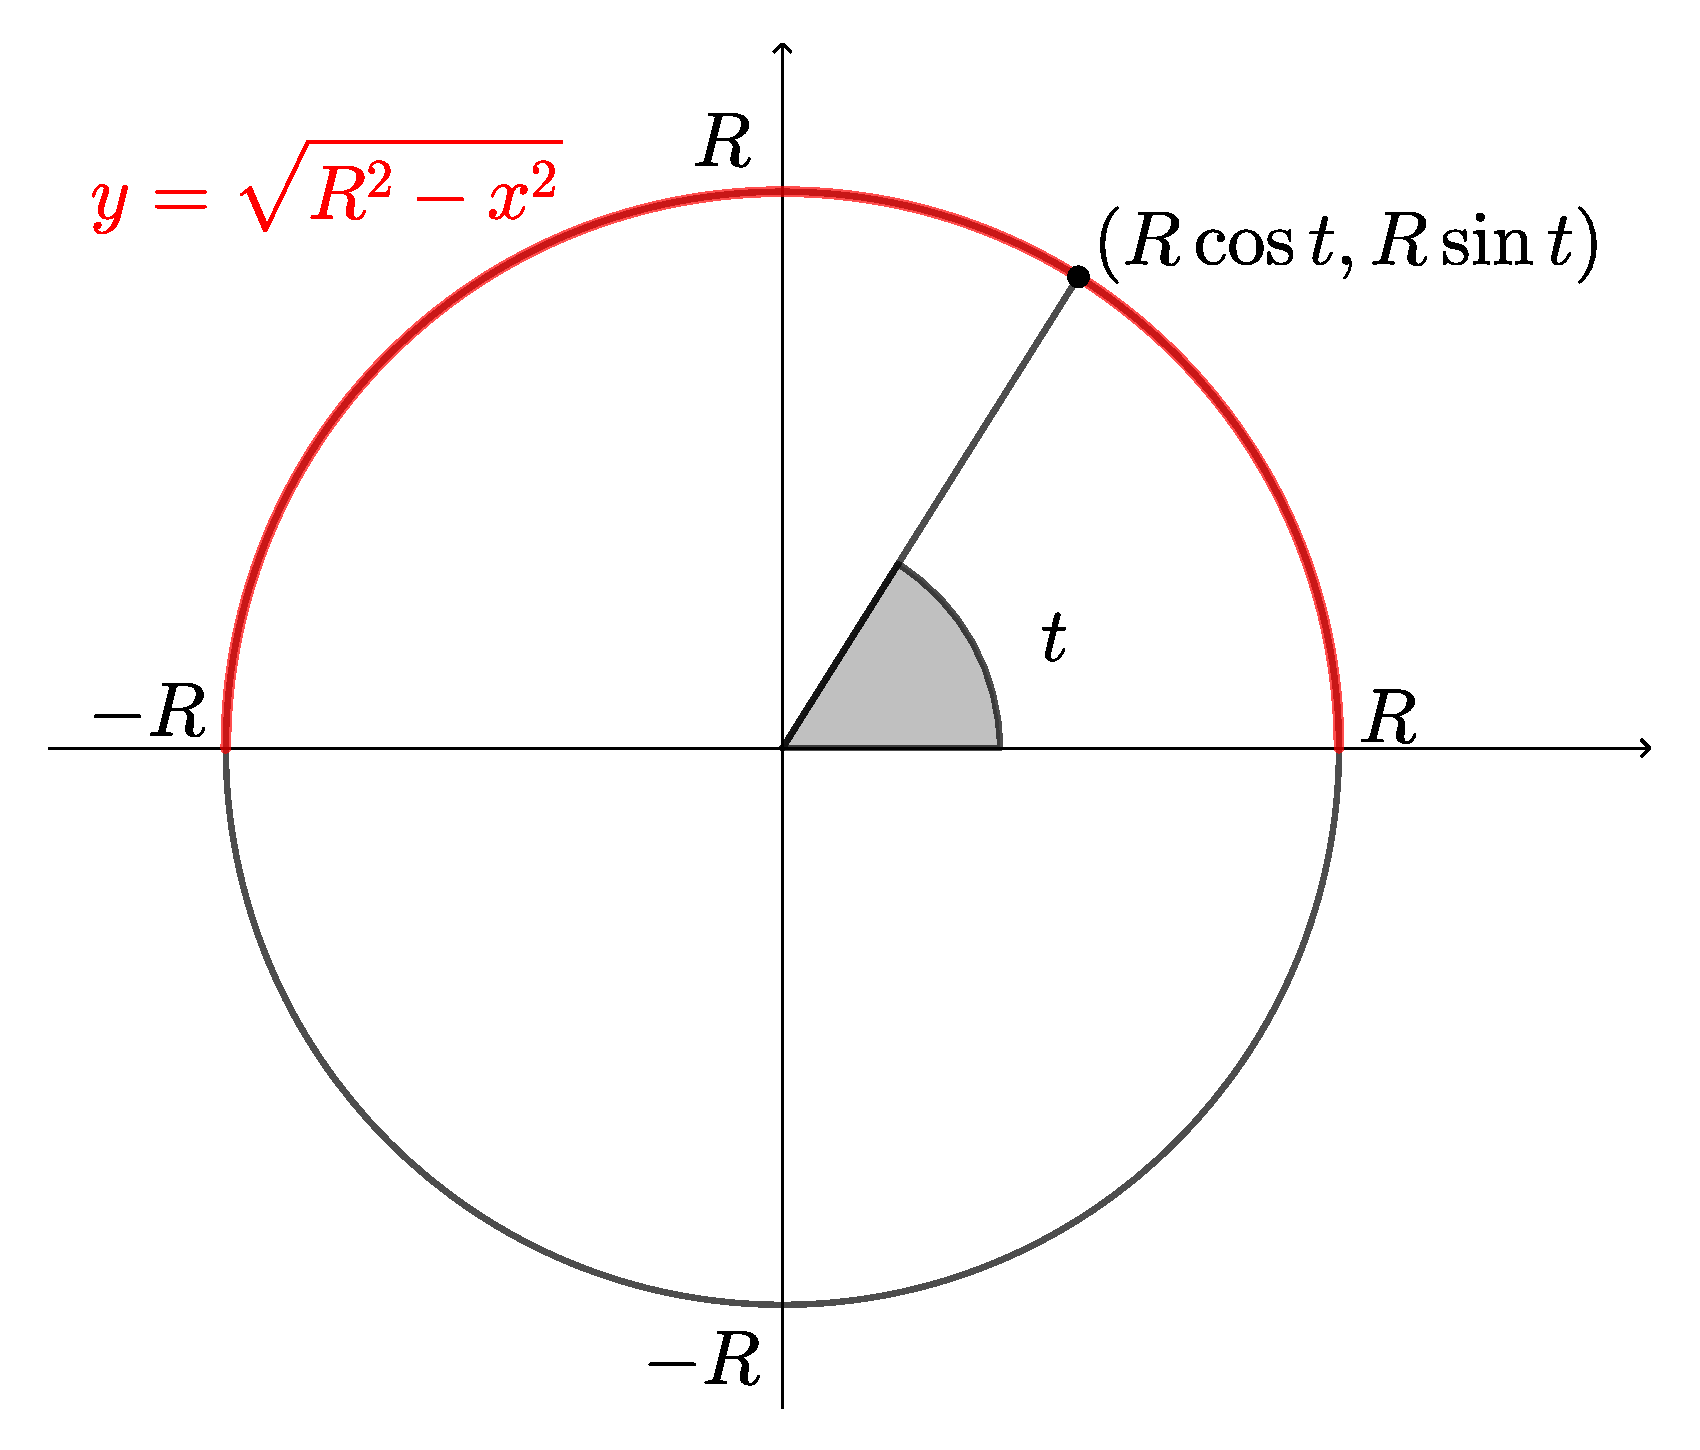
\includegraphics[height=5cm]{05/circle_par.pdf}
    \caption{}
    \label{fig:circle_par}
  \end{figure}
  
  
\end{example}

\begin{example}\label{exmp:parab-length}
  放物線 $y=x^2$ の $0 \leqq x \leqq 1$ の部分の長さ $L$ は定理\ref{thm:lengraph}より以下のように求められる.
  \[
    \begin{aligned}
      L&=\int_{0}^{1} \sqrt{ 1 + \left( \left( x^2\right)'\right)^2}\ dx 
         = \int_{0}^{1} \sqrt{1+4x^2}\ dx
         = \frac{1}{2}\left[ x \sqrt{1+4x^2} + \frac{1}{2} \log \left( 2x+\sqrt{1+4x^2}\right)\right]_{0}^{1}\\
       & = \frac{\sqrt{5}}{2} + \frac{1}{4} \log \left( 2+\sqrt{5} \right)
    \end{aligned}
  \]
  \begin{figure}[h]
    \centering
    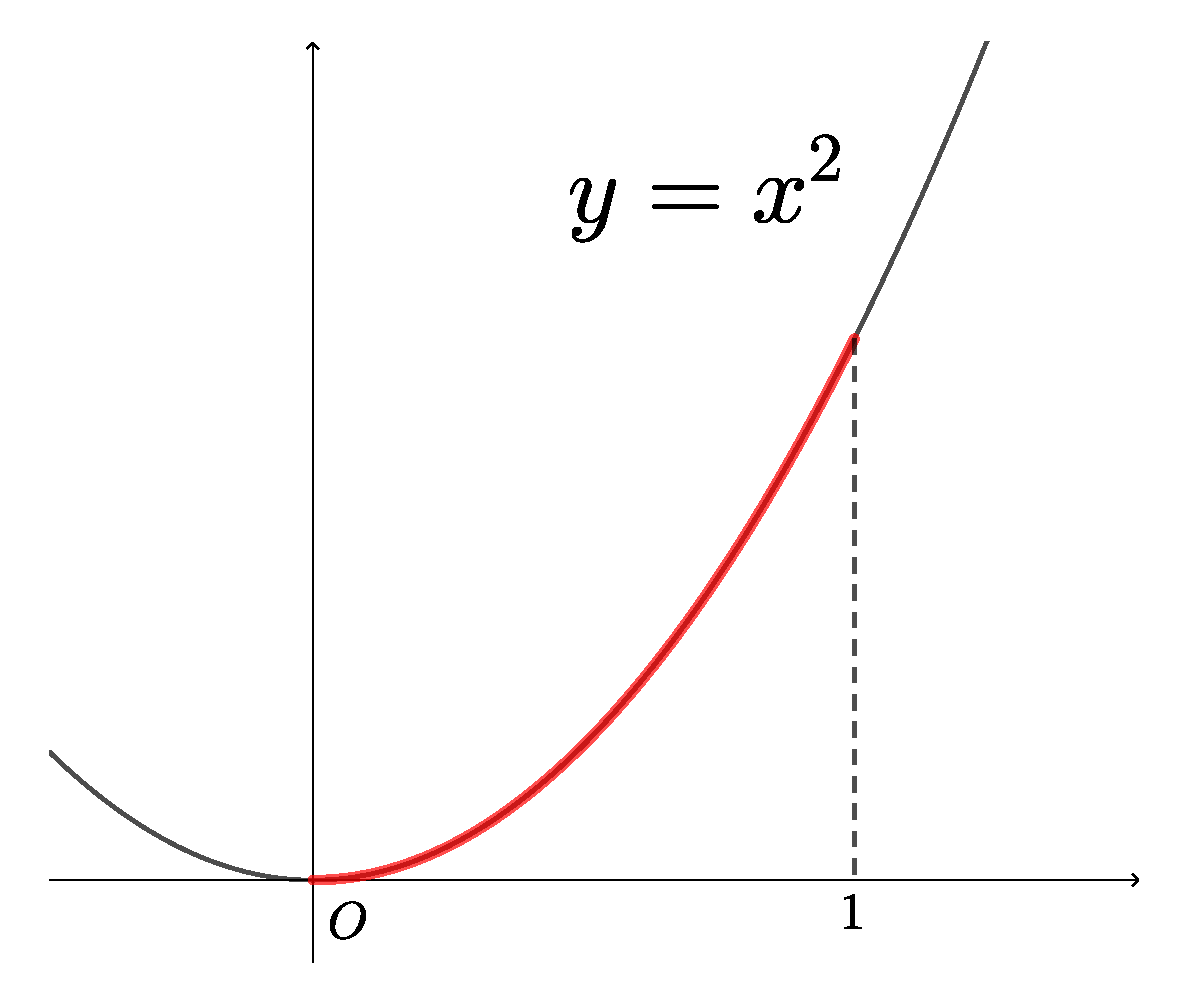
\includegraphics[height=5cm]{05/parab.pdf}
    \caption{放物線 $y=x^2$}
  \end{figure}
\end{example}

\newpage

\subsection{空間曲線の長さと積分}

$\varphi, \psi, \chi$ を閉区間 $[a,b]$ 上定義された $C^1$ 級関数とする.
変数 $t$ が $a$ から $b$ まで動くとき,空間の点 $(\varphi(t), \psi(t),
\chi(t))$ はなめらかな空間曲線 $C$ を描く.これを
\[
  x=\varphi(t), \quad y=\psi(t), \quad z=\chi(t), \quad a \leqq t \leqq b
\]
と書き,空間曲線 $C$ の媒介変数表示という.平面曲線と同様に,空間曲線 $C$ の長さは以下の
積分に等しい.
\[
  \int_{a}^{b} \sqrt{ {\varphi'(t)}^2 + {\psi'(t)}^2 + {\chi'(t)}^2} \ dt
\]

\begin{example}
  常螺旋曲線
  \[
    x=\cos t, \; y=\sin t, \; z=t, \; 0 \leqq t \leqq 2\pi
  \]
  の長さは以下の積分で求められる.
  \begin{align*}
    \int_{0}^{2\pi} \sqrt{ \left( \left( \cos t\right)'\right)^2 + \left( \left( \sin t\right)'\right)^2 
        + \left( t'\right)^2} \ dt
        = \int_{0}^{2\pi} \sqrt{2} \ dt = 2\sqrt{2} \pi
  \end{align*}
  \begin{figure}[h]
    \centering
    \includegraphics[width=10cm]{05/spiral.png}
  \end{figure}
\end{example}

平面曲線は $\bm{r}(t) = \left( x(t), y(t) \right)$ と表せる.また,空間
曲線は $\bm{r}(t) = \left( x(t), y(t), z(t)\right)$ と表せる.平面曲線
に対して $\bm{r}'(t)=\left( x'(t), y'(t)\right)$ とし,空間曲線に対し
て $\bm{r}'(t)=\left( x'(t), y'(t), z'(t)\right)$ とすれば,いずれもの
その長さは以下のように統一的に表せる.
\[
  \int_{a}^{b} \left| \bm{r}'(t)\right| \ dt
\]

\subsection{練習問題}

\begin{enumerate}

\item 曲線 $y=\sin x$ と $y=\cos x$ で囲まれる下図斜線部分の図形の
  面積を求めよう.
  \begin{figure}[h]
    \centering
    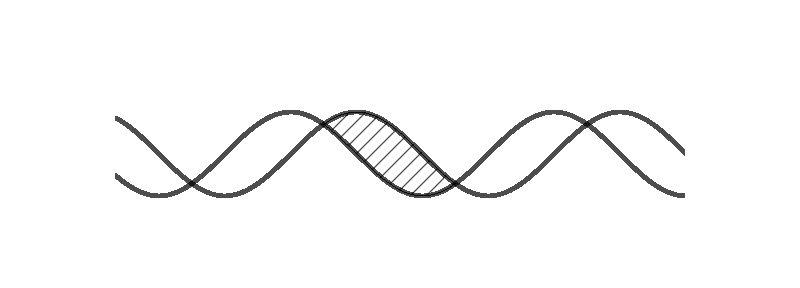
\includegraphics[height=4.5cm]{05/sincos.pdf}
  \end{figure}
  
\item 次の曲線の長さを求めよう.
  \vspace{1zh}
  
  \begin{enumerate}[(1)]

    
  \item $\begin{cases}
      x=t-\sin t\\
      y=1-\cos t
    \end{cases}\quad (0 \leqq t \leqq \pi)$
    \begin{figure}[h]
      \centering
      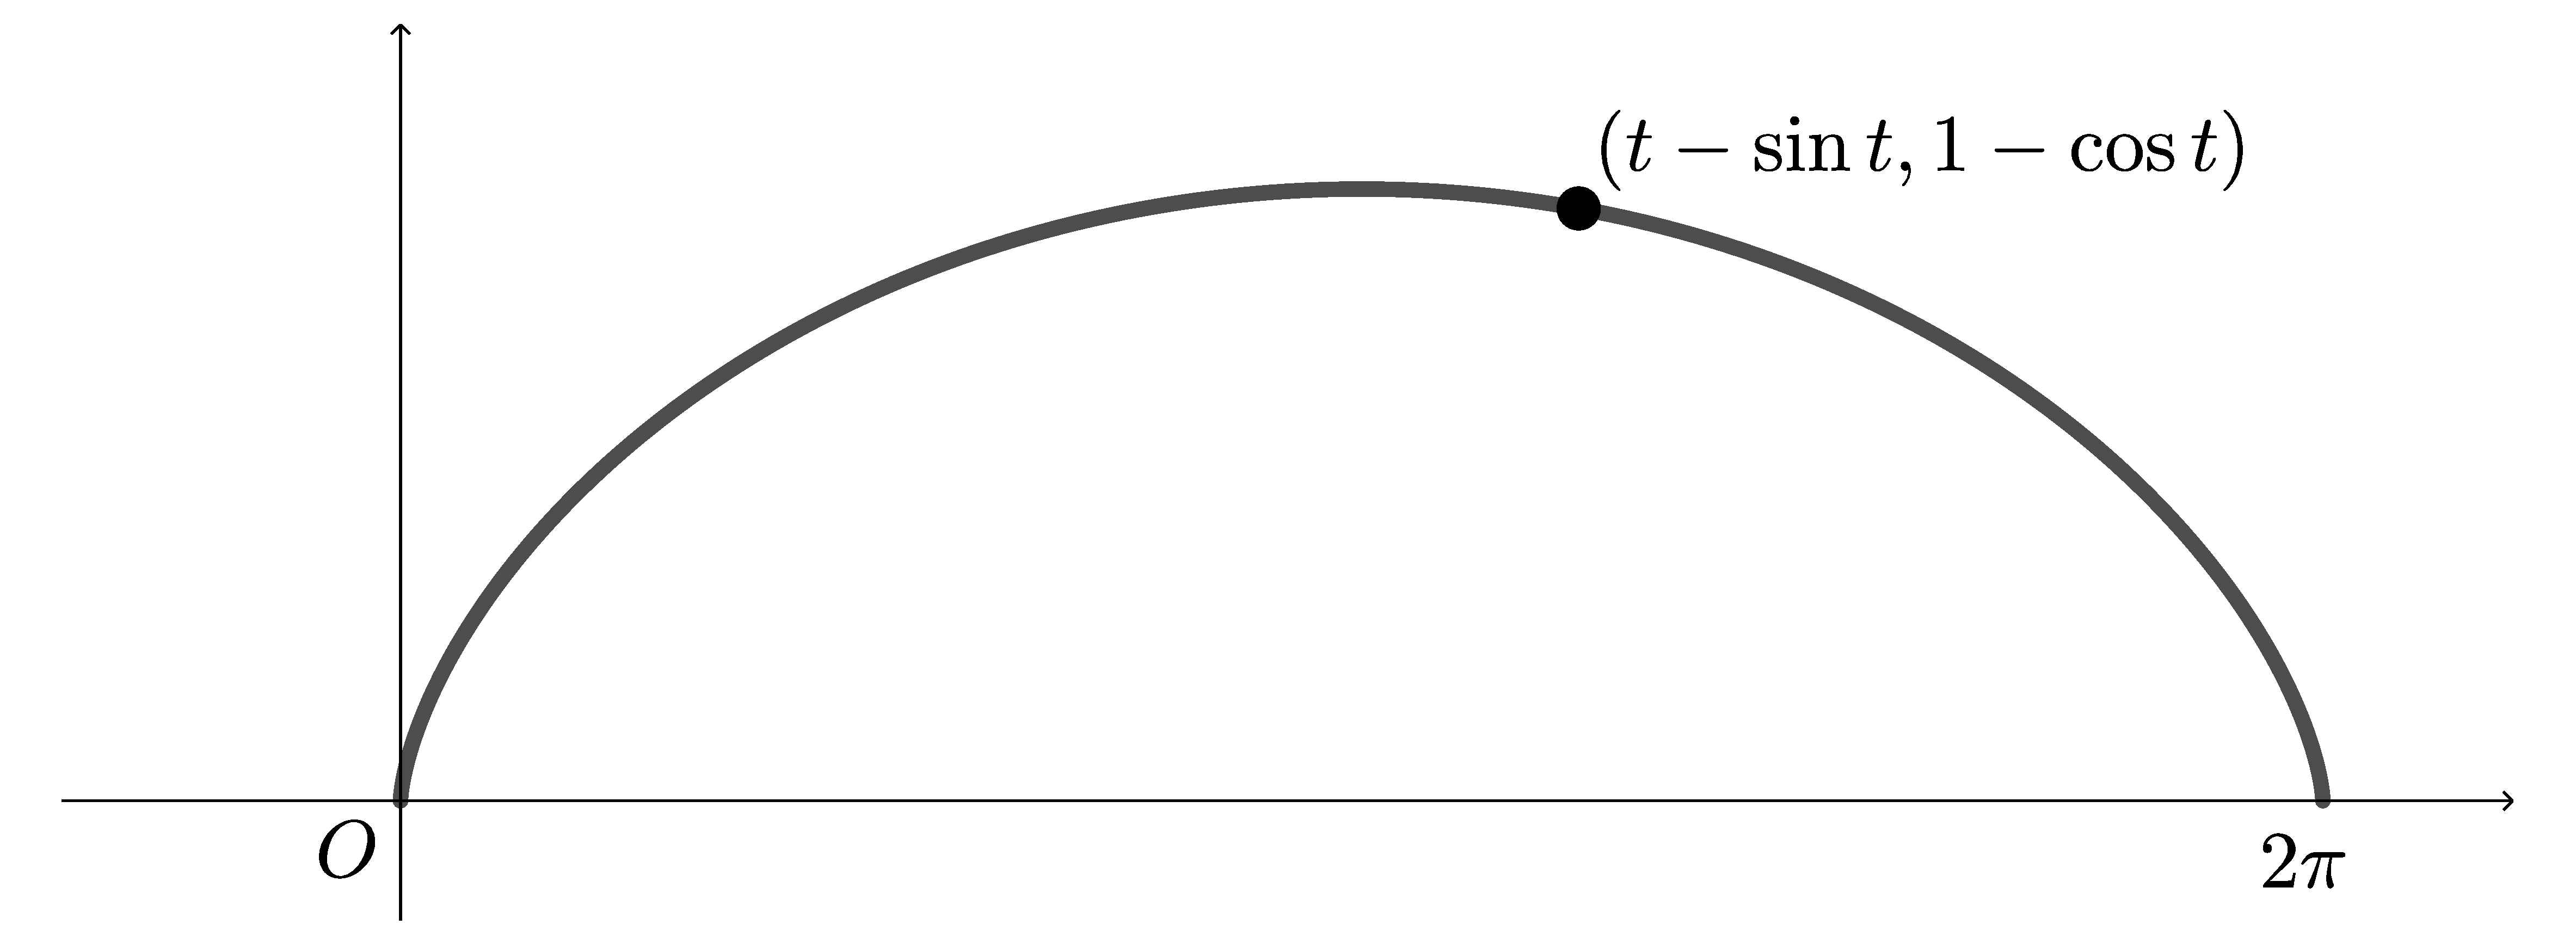
\includegraphics[height=4.5cm]{05/cycloid.pdf}
    \end{figure}
    
  \item $\ds y=\frac{e^{x}+e^{-x}}{2} \; \left(= \cosh x\right) \quad (0 \leqq x \leqq \log 2)$
    \begin{figure}[h]
      \centering
      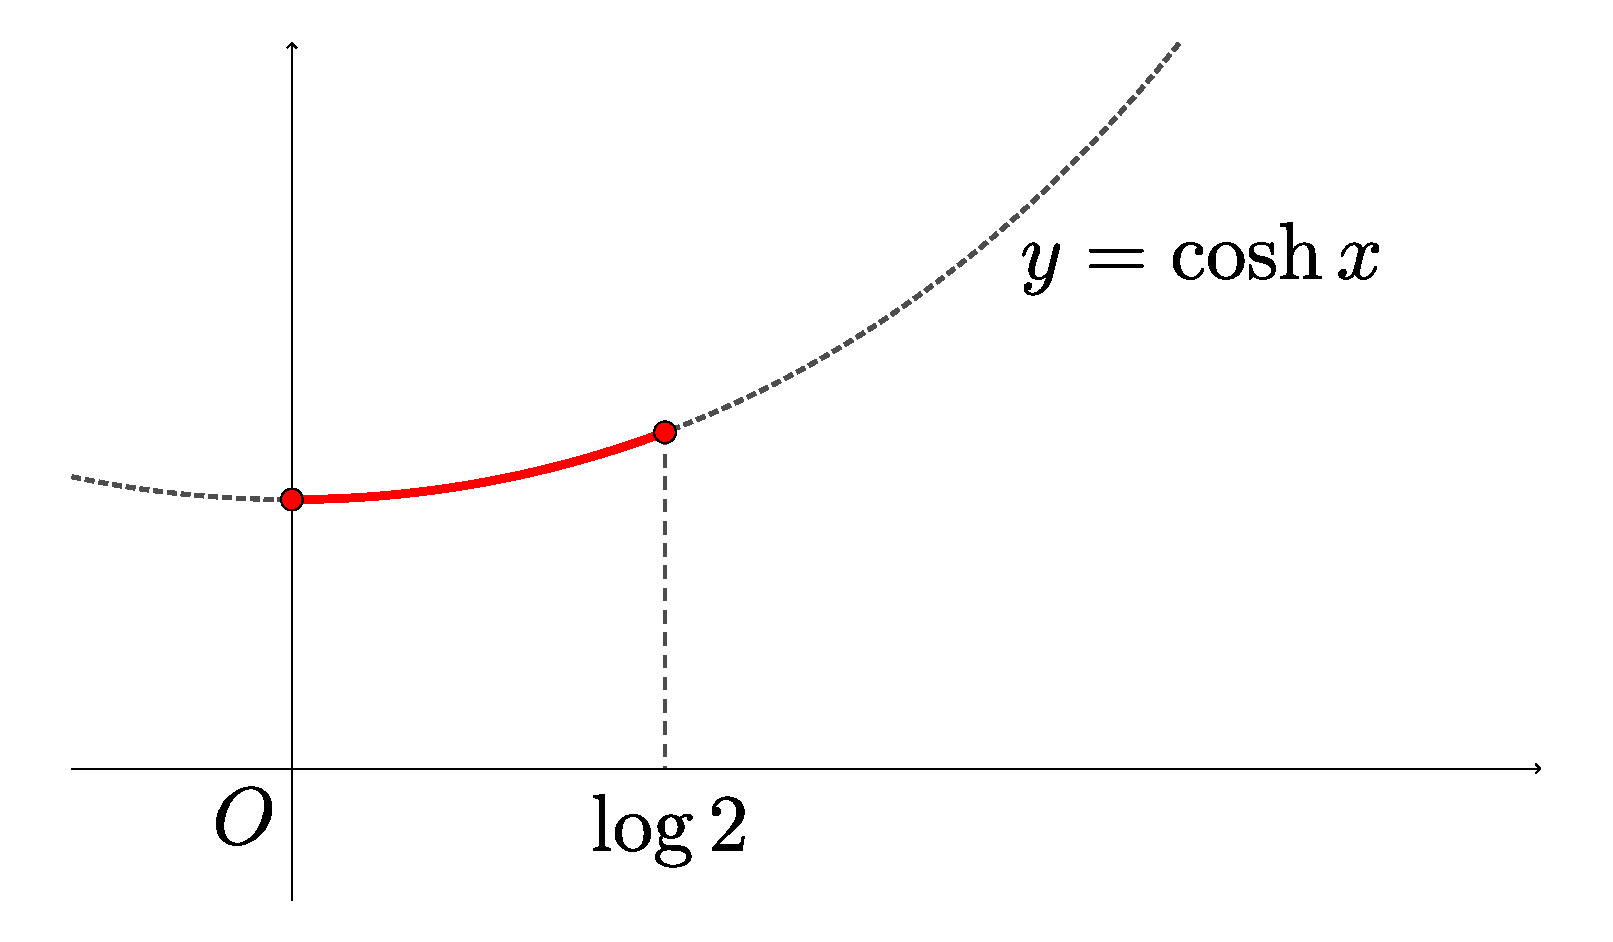
\includegraphics[height=4.5cm]{05/cosh.pdf}
    \end{figure}
  \end{enumerate}
  
  \begin{figure}[b]
  答え : 1. $2\sqrt{2}$ \qquad 2. (1) $4$ \quad (2) $\frac{3}{4}$
\end{figure}

\end{enumerate}

\subsection{(おまけ)平方根を含む関数の積分と双曲線関数}

例えば
\[
  \int \frac{dx}{\sqrt{a^2+x^2}} \quad \text{ や } \quad \int \sqrt{a^2+x^2} \ dx
\]
ような平方根を含む関数の積分には,$u=x+\sqrt{a^2+x^2}$ とおいて置換積
分を使うという自力で見出すのはやや困難な方法がある.それを紹介してもよ
いが,どうせならより自力で見出しにくい方法を紹介しておく.\\

以下の $3$ 個の関数は\textbf{双曲線関数}と呼ばれる.
\[
  \sinh x := \frac{e^{x}-e^{-x}}{2} \qquad \cosh x := \frac{e^{x}+e^{-x}}{2} \qquad
  \tanh x:=\frac{\sinh x}{\cosh x} = \frac{e^{x}-e^{-x}}{e^{x}+e^{-x}}
\]
それぞれ,hyperbolic sine, hyperbolic cosine, hyperbolic tangent と読む.
三角関数の記号 $\sin, \cos, \tan$ とよく似ているが全く別の関数である.
それでいて三角関数に非常によく似た性質を持っている.例えば
\[
  \cosh^2 x - \sinh^2 x =1, \qquad 1 - \tanh^2 x = \frac{1}{\cosh^2x}
\]
という関係式が成り立つことが定義から容易に確かめられる.さらには,三角
関数の加法定理によく似た公式
\[
  \sinh(x \pm y) = (\sinh x)(\cosh y) \pm (\cosh x)(\sinh y), \quad
  \cosh(x \pm y) = (\cosh x)(\cosh y) \pm (\sinh x)(\sinh y)
\]
を定義から容易に導ける.符号の反転が起こらないので,三角関数の公式より
も覚えやすい.三角関数の加法定理が倍角・半角の公式を導くのと全く同様に,
これらは双曲線関数に関する類似の公式
\[
  \begin{aligned}
    &\sinh(2x) = 2 (\sinh x)(\cosh x), \qquad \cosh(2x) = \cosh^2 x +
      \sinh^2 x = 2\cosh^2 x -1 = 1+2\sinh^2 x\\[1ex]
    &\cosh^2(x) = \frac{1+\cosh(2x)}{2}, \qquad \sinh^2 x = \frac{\cosh(2x)-1}{2}
  \end{aligned}
\]
などを導く.さらには,各々の導関数に関しても
\[
  \left( \sinh x \right) = \cosh x, \quad \left( \cosh x \right)' = \sinh x, \quad
  \left( \tanh x\right)' = \frac{1}{\cosh^2x} = 1 - \tanh^2 x
\]
となることもやはり定義から容易に確認できる.これらから積分の公式
\[
  \int \sinh x \ dx = \cosh x, \quad \int \cosh x \ dx = \sinh x,
  \quad \int \frac{dx}{\cosh^2 x} = \tanh x
\]
も導かれる.いずれも三角関数間の関係式とよく似ているが,符号の反転が起きないので覚えやすい.\\

また,逆三角関数が $\sin^{-1}, \cos^{-1}, \tan^{-1}$ と書かれるように,
双曲線関数においても $\sinh^{-1}, \cosh^{-1}, \tanh^{-1}$ は逆数ではな
く,各々の逆関数を表す.その導関数は逆関数の微分公式を使って逆三角関数
と同様に計算できる.例えば $y=\sinh^{-1}x$ の導関数であれば,$x=\sinh
y$ なので
\[
  \left( \sinh^{-1}x \right)'= \frac{dy}{dx} = \frac{1}{\frac{dx}{dy}}
  = \frac{1}{\cosh y} = \frac{1}{\sqrt{1+\sinh^2y}} =
  \frac{1}{\sqrt{1+x^2}}
\]
と計算できる.これは以下の積分の公式を導く.
\[
  \int \frac{dx}{\sqrt{1+x^2}} = \sinh^{-1}x \quad \Bigg( = \log \left( x + \sqrt{1+x^2}\right) \Bigg)
\]
\newpage

長々と語った双曲線関数の一連の性質を使って,例として以下の積分公式を導出する.
\begin{equation}\label{eq:int-sqrt-sinh}
  \int \sqrt{a^2+x^2} \ dx = \frac{1}{2}\left( a^2 \log \left(x+\sqrt{a^2+x^2}\right) + x \sqrt{a^2+x^2} \right) \quad (a>0)
\end{equation}
突然だが
$\ds x= a \sinh u \; \left( \Leftrightarrow u =
  \sinh^{-1}\frac{x}{a}\right)$ とおく.$\ds \frac{dx}{du} = a \cosh
u$ なので
\begin{equation}\label{eq:x-asinh}
  \begin{aligned}
    \int \sqrt{a^2+x^2} \ dx
    &= \int a \sqrt{1+\sinh^2 u}~ \frac{dx}{du}\ du
      = \int a \sqrt{\cosh^2 u}~ \left( a \cosh u\right) \ du
      = a^2 \int \cosh^2 u \ du\\[1ex]
    &= a^2 \int \frac{1+\cosh(2u)}{2} \ du = a^2\left( \frac{u}{2} + \frac{1}{4}\sinh(2u) \right)
      = a^2 \left( \frac{u}{2} + \frac{(\sinh u)(\cosh u)}{2}\right)\\[1ex]
    & = \frac{a^2}{2}\left( u + \left( \sinh u\right) \sqrt{1+\sinh^2 u}\right)
      =\frac{a^2}{2}\left( \sinh^{-1}\frac{x}{a} + \frac{x}{a} \sqrt{1+ \left(\frac{x}{a}\right)^2}\right)\\[1ex]
    & = \frac{1}{2}\left( a^2 \sinh^{-1}\frac{x}{a} + x \sqrt{a^2+x^2}\right)
  \end{aligned}
\end{equation}
である.前ページで紹介した諸々の公式を随所で使いまくっている.ここで,$\ds y=\sinh^{-1}\frac{x}{a}$ とおけば
\[
  y = \sinh^{-1}\frac{x}{a} \; \Longleftrightarrow \; \frac{x}{a} =
  \sinh y = \frac{e^{y}-e^{-y}}{2} \; \Longleftrightarrow \;
  a \left( e^y\right)^2 -2x e^y - a=0
\]
である.最後の等式を $e^y$ に関する2次方程式として解けば,$e^y >0$ と合わせて
\[
  e^y = \frac{x + \sqrt{a^2+x^2}}{a} \quad \text{ より }  \quad y = \log \left( x + \sqrt{a^2+x^2}\right) - \log a
\]
である.(\ref{eq:x-asinh})の最後の $\ds \sinh^{-1}\frac{x}{a}$ をこ
の $y$ に置き換えて,定数 $\ds -\frac{a^2}{2}\log a$ を積分定数に吸収させれば (\ref{eq:int-sqrt-sinh}) が得られる.\\

例\ref{exmp:parab-length}で以下の積分公式をさりげなく使った.
\[
  \int \sqrt{1+4x^2} \ dx = \frac{1}{2}\left(\frac{1}{2} \log \left( 2x + \sqrt{1+4x^2}\right) + x \sqrt{1+4x^2}\right)
\]
これは(\ref{eq:int-sqrt-sinh}) で $\ds a=\frac{1}{2}$ とすれば得られる.実際,
\[
  \int \sqrt{ \left( \frac{1}{2}\right)^2 + x^2 } \ dx = \int
  \sqrt{\frac{1+4x^2}{4}} \ dx = \frac{1}{2}\int \sqrt{1+4x^2} \ dx
\]
なので,$\ds a=\frac{1}{2}$ のときの(\ref{eq:int-sqrt-sinh})を $2$ 倍す
ればよい.なお,定数の差は積分定数が吸収してくれる.\\

この他にも双曲線関数によって計算しやすくなる積分がいくつかある.双曲線
関数やそれにまつわる積分についてより詳しく知りたければ以下の記事を読ん
でみてください.
\begin{center}
  双曲線関数について : \url{https://github.com/kazutsumi/hyperbolic/blob/main/hyperbolic.pdf}
\end{center}



\end{document}
